\documentclass[10pt,aspectratio=169]{beamer}

\usetheme{Madrid}
\usecolortheme{default}

\usepackage[utf8]{inputenc}
\usepackage[T1]{fontenc}
\usepackage[french]{babel}
\usepackage{amsmath,amssymb}
\usepackage{graphicx}
\usepackage{booktabs}
\usepackage{tabularx}
\usepackage{array}
\usepackage{xltabular}
\usepackage[authoryear,round]{natbib}

\title[Détection de deepfakes]{Détection de deepfakes générés par des modèles de diffusion}
\author[A. Mugisha, V. Pedoussat]{Axcel Mugisha \and Victoria Pedoussat}
\institute[IMT]{
IMT -- Université de Toulouse\\
\texttt{axcel.mugisha@utoulouse.fr}\\
\texttt{victoria.pedoussat@utoulouse.fr}
}
\date{\today}

\begin{document}

\begin{frame}
  \titlepage
\end{frame}


\begin{frame}{Plan}
  \tableofcontents[hideallsubsections]
\end{frame}
%%%%%%%%%%%%%%%%%%%%%%%%%%%%%%%%%%%%%%%%%%%%%%%%%%%%%%%%%%%%%%%%%%%%%%
\section{Introduction}
\begin{frame}{Contexte et problématique}

\textbf{Constat.}
Les modèles génératifs récents, en particulier les modèles de diffusion, produisent des images et vidéos de plus en plus réalistes.

\vspace{0.4cm}

\textbf{Problème.}
Les détecteurs classiques apprennent souvent des artefacts visibles ou propres à un générateur donné, mais généralisent mal à de nouveaux modèles.

\vspace{0.4cm}

\textbf{Question centrale.}
$$
    f(x) \rightarrow \{\text{réel}, \text{généré}\}
$$

\begin{block}{Défi principal}
Construire des méthodes capables de détecter des contenus générés par des modèles inconnus, même après compression, redimensionnement ou dégradation.
\end{block}

\end{frame}


\begin{frame}{Pourquoi exploiter la reconstruction ?}

\begin{block}{Hypothèse}
Une image générée est souvent plus proche de la distribution apprise par un modèle génératif qu’une image réelle capturée par caméra.
\end{block}

\begin{figure}
    \centering
    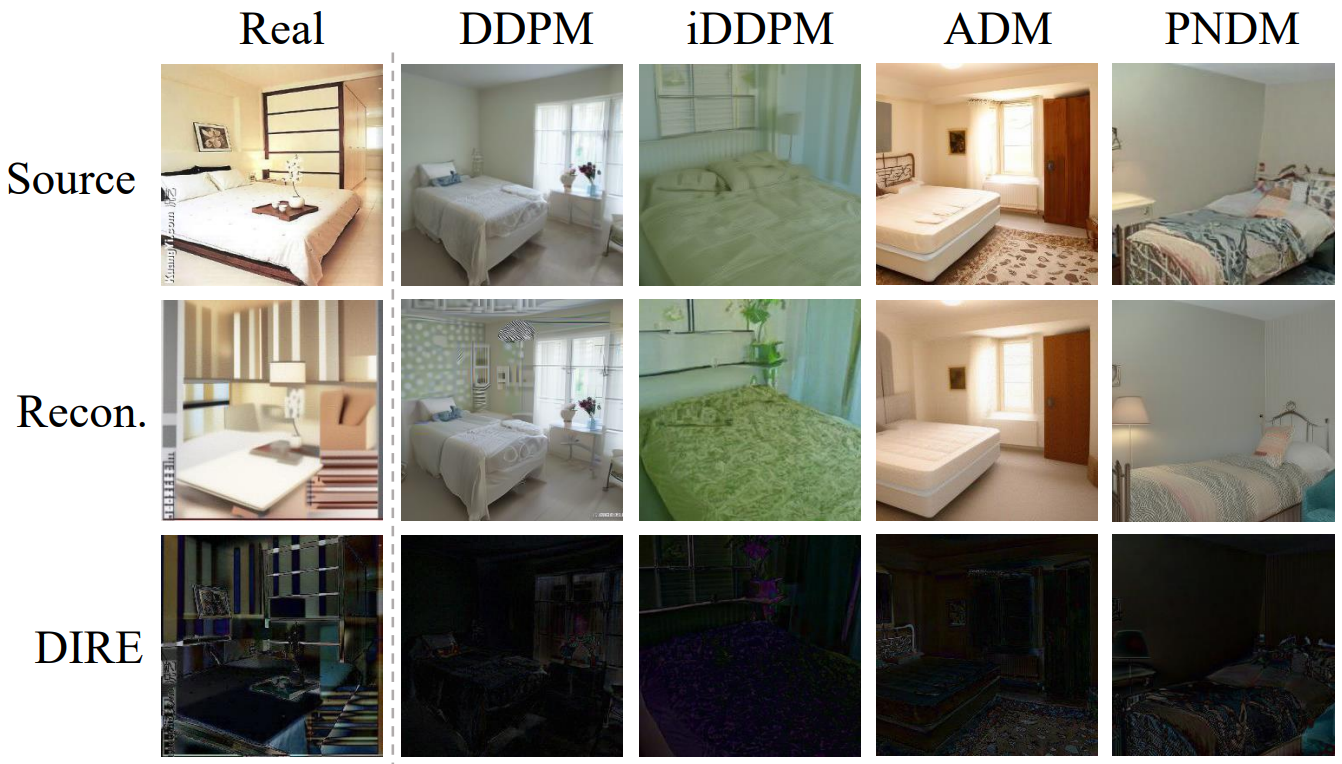
\includegraphics[width=0.4\linewidth]{Dire_teaser.png}
    \caption{ Exemples des erreurs de reconstructions  d'une image réelle et des images générées par des models de diffusion: DDPM \citep{NEURIPS2020_4c5bcfec}, iDDPM \citep{nichol2021improveddenoisingdiffusionprobabilistic}, ADM \citep{dhariwal2021diffusionmodelsbeatgans}, et PNDM \citep{liu2022pseudonumericalmethodsdiffusion} respectivement, obtenues en utilisant la méthode DIRE (voir slide suivante). }
    \label{fig:placehold}
\end{figure}
\end{frame}


%%%%%%%%%%%%%%%%%%%%%%%%%%%%%%%%%%%%%%%%%%%%%%%%%%%%%%%%%%%%%%%%%%%%%%%%%

\section{Méthodes de détection}
\subsection{DIRE}
\begin{frame}{DIRE : Diffusion Reconstruction Error \citep{wang2023dirediffusiongeneratedimagedetection}}

\textbf{Idée principale.}
Reconstruire une image avec un modèle de diffusion pré-entraîné, puis comparer l’image originale et sa reconstruction.


$$
    x \longrightarrow \hat{x}=R_{\text{diff}}(x) ,\quad  \text{et l'erreur de reconstruction} \quad E_{\text{DIRE}}(x)=|x-\hat{x}|
$$

\begin{figure}
    \centering
    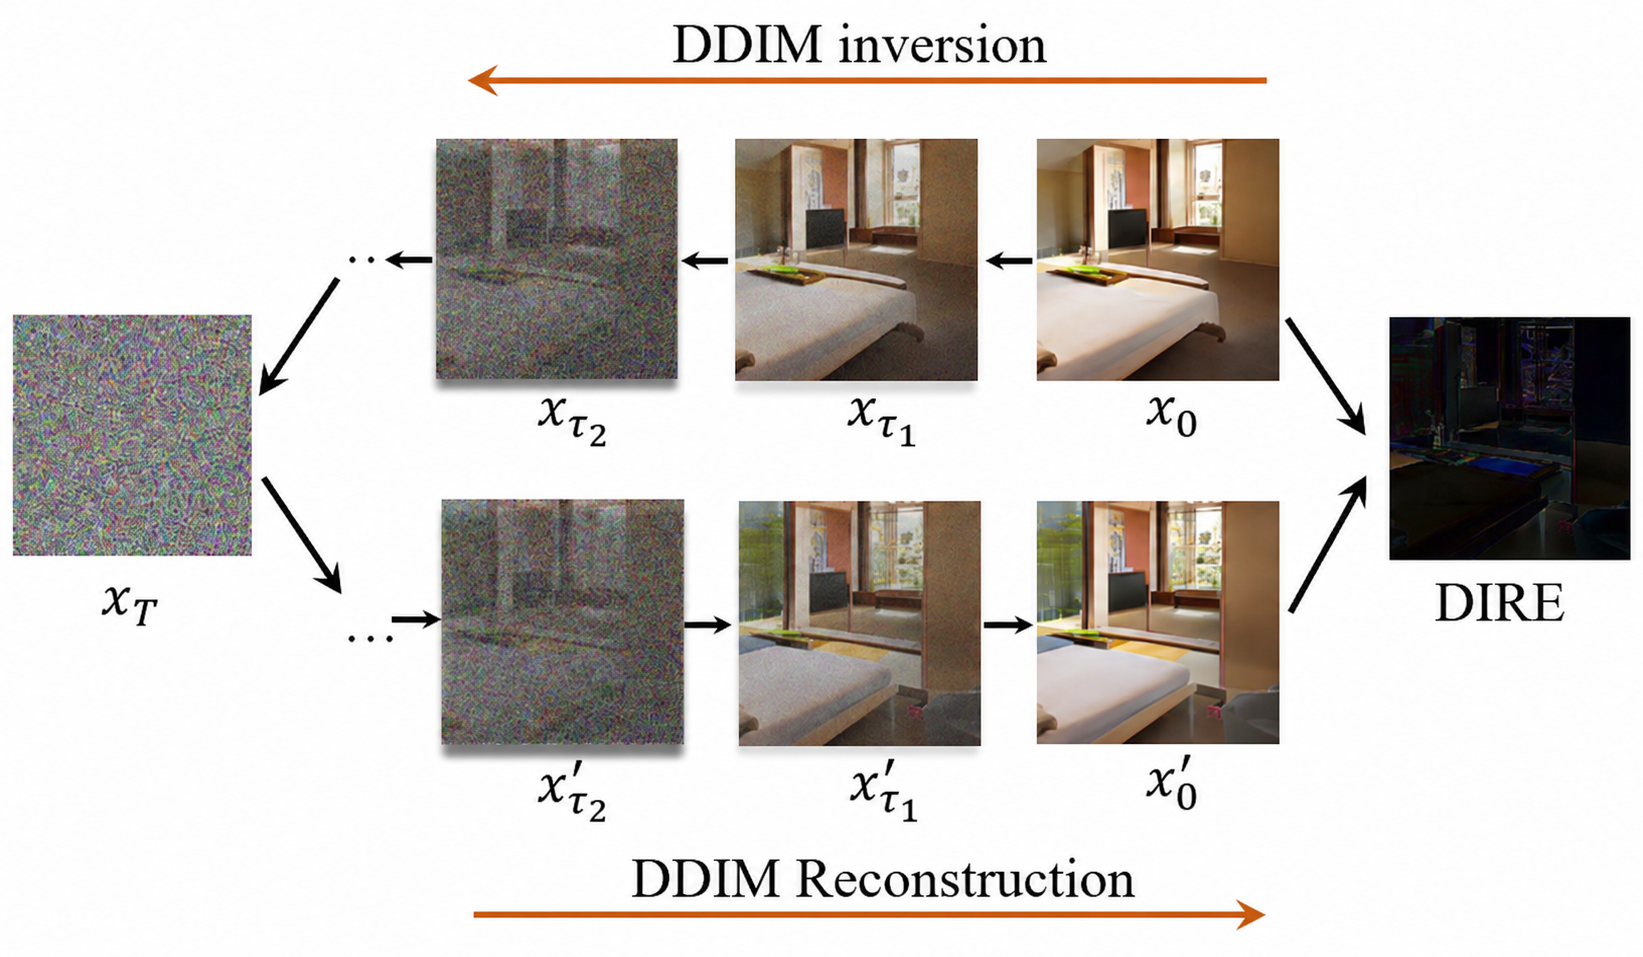
\includegraphics[width=0.4\linewidth]{dire_cleaned.png}
    \caption{\textbf{Calcul de DIRE à partir d’une image d’entrée $x_0$}. L’image est d’abord inversée en bruit $x_T$, puis reconstruite par débruitage progressif (inversion DDIM \citep{song2022denoisingdiffusionimplicitmodels}). DIRE est défini comme le résidu entre l’image originale $x_0$ et l’image reconstruite $x'_0$.}
    \label{fig:placeholder}
\end{figure}

\end{frame}


\subsection{SeDID}
\begin{frame}{SeDID : Stepwise Error \citep{ma2023exposingfakeeffectivediffusiongenerated}}

\textbf{Idée principale.}
Exploiter une erreur intermédiaire dans le processus de diffusion, plutôt qu’une reconstruction finale. On estime d'abord l'image propre
$$
    f_\theta(x,t)=\frac{x-\sqrt{1-\bar{\alpha}_t}\varepsilon_\theta(x,t)}{\sqrt{\bar{\alpha}_t}}
$$
Et on définit  deux fonctions: la fonction de débruitage qui permet de passer d'un timestep $t$ à $t-\delta$
$$
    \psi_\theta(x,t,\delta)=\sqrt{\bar{\alpha}_{t-\delta}}f_\theta(x,t)+\sqrt{1-\bar{\alpha}_{t-\delta}}\varepsilon_\theta(x,t)
$$
Et la fonction reverse qui permet de passer d'un timestep $t$ à $t+\delta$
$$
    \phi_\theta(x,t,\delta)=\sqrt{\bar{\alpha}_{t+\delta}}f_\theta(x,t)+\sqrt{1-\bar{\alpha}_{t+\delta}}\varepsilon_\theta(x,t)
$$
Ainsi, l'erreur de reconstruction devient
$$
    E_{t,\delta}
=
\left\|
\psi_\theta
\left(
\phi_\theta(\tilde{x}_t,t,\delta),
t,\delta
\right)
-
\tilde{x}_t
\right\|^2
$$
\end{frame}
\begin{frame}{SeDID (suite)}
    \begin{figure}
    \centering
    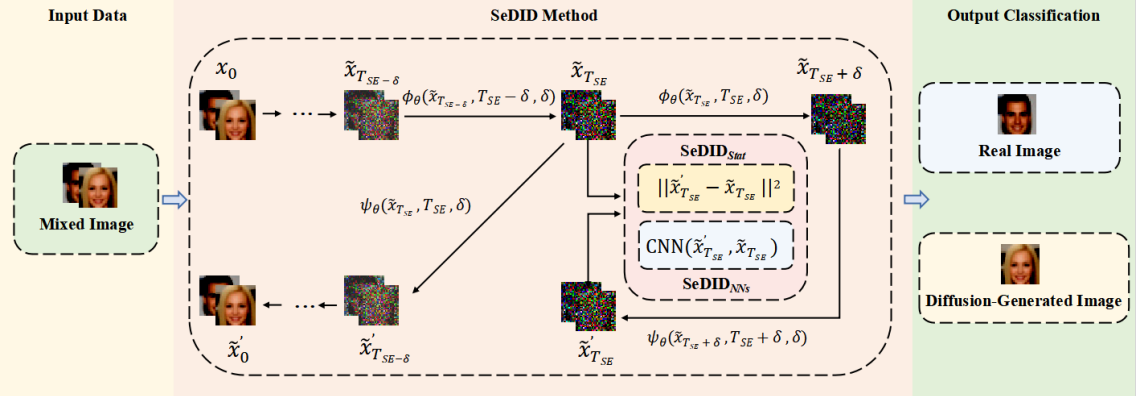
\includegraphics[width=1
    \linewidth]{SeDID.png}
    \caption{\textbf{Pipeline de la méthode SeDID}. À partir d’un ensemble d’images réelles et synthétiques, SeDID extrait un profil de bruit permettant de caractériser les images générées par diffusion. La méthode se divise ensuite en deux branches : une approche statistique, $\text{SeDID}_{\text{Stat}}$, basée sur l’analyse des erreurs, et une approche par réseau de neurones, $\text{SeDID}_{\text{NNs}}$, utilisant un ResNet entraîné par rétropropagation.}
    \label{fig:placeholder}
\end{figure}
\end{frame}


\subsection{AEROBLADE}
\begin{frame}{AEROBLADE : Autoencoder Reconstruction Error \citep{ricker2024aerobladetrainingfreedetectionlatent}}

\textbf{Idée principale.}
Utiliser l’autoencodeur d’un modèle de diffusion latente pour reconstruire l’image.

$$
    z=\mathcal{E}(x)
\qquad
\hat{x}=\mathcal{D}(z)=\mathcal{D}(\mathcal{E}(x)), \text{ ainsi}
\quad E_{\text{AE}}(x)=|x-\mathcal{D}(\mathcal{E}(x))|
$$
\begin{figure}
    \centering
    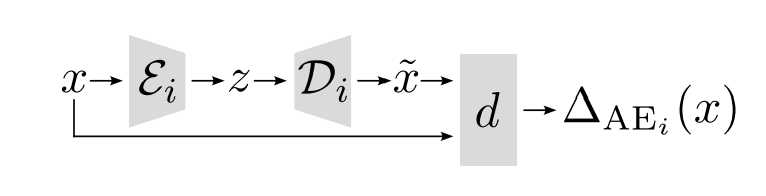
\includegraphics[width=0.5\linewidth]{aeroblade.png}
    \caption{\textbf{Illustration de la méthode AEROBLADE}. L’erreur de reconstruction $\Delta_{\text{AE}_i}(x)$ mesure la différence entre l’image originale $x$ et l’image reconstruite $\tilde{x}$, après passage dans l’encodeur $\mathcal{E}_i$ et le décodeur $\mathcal{D}_i$ d’un autoencodeur de modèle de diffusion latente.}
    \label{fig:placeholder}
\end{figure}
\end{frame}

\subsection{LaRE\textsuperscript{2}}
\begin{frame}{LaRE\textsuperscript{2} : erreur de reconstruction latente \citep{10656812}}

\textbf{Idée principale.}
Mesurer l’erreur de reconstruction non pas dans l’image, mais dans l’espace latent, puis l’utiliser pour guider les features visuelles.
$$
z=\mathcal{E}(x),\text{et}
\quad z_t=\sqrt{\alpha_t}z+\sqrt{1-\alpha_t}\varepsilon
$$
On utilise un U-Net pour prédire le bruit quia été ajouté à $z$:
$$
    \hat{\varepsilon}_\theta=\varepsilon_\theta(z_t,t)
$$
Et on déduit le latent propre:
$$
    \hat{z}=\frac{z_t-\sqrt{1-\alpha_t}\hat{\varepsilon}_\theta}{\sqrt{\alpha_t}}
    \qquad
    E_{\text{LaRE}}(x)=|z-\hat{z}|
$$
La carte d’erreur latente est combinée aux features extraites par un backbone :
$$
    F=B(x),\qquad \tilde{E}_{\text{LaRE}}=A(E_{\text{LaRE}})
$$
$$
    F_{\text{refined}}=\operatorname{EGRE}(F,\tilde{E}_{\text{LaRE}})
$$
\end{frame}
\begin{frame}{LaRE\textsuperscript{2} (suite)}
    \begin{figure}
        \centering
        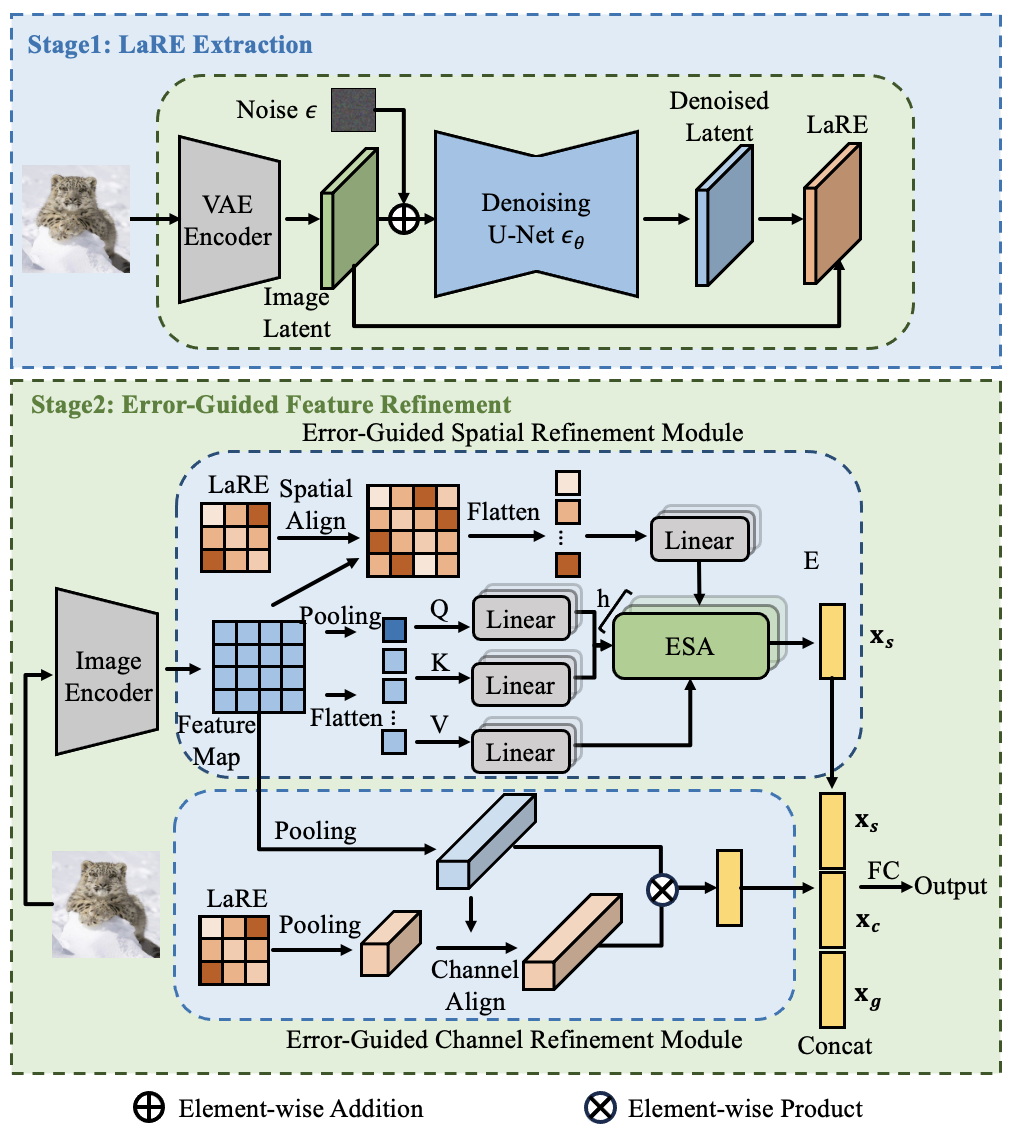
\includegraphics[width=0.3\linewidth]{Lare2.png}
        \caption { La méthode LaRE² extrait d’abord une carte d’erreur LaRE dans l’espace latent, puis utilise cette erreur pour dire au détecteur où regarder dans l’image et quels canaux de caractéristiques sont importants pour distinguer une image réelle d’une image générée(la méthode EGRE).}
        \label{fig:placeholder}
    \end{figure}
\end{frame}


\subsection{DRCT}
\begin{frame}{DRCT : Diffusion Reconstruction Contrastive Training \citep{chen2024drct}}

\textbf{Idée principale.}
Utiliser les images reconstruites par diffusion comme exemples supplémentaires pour apprendre de meilleures représentations.

\vspace{0.25cm}

$$
    x \longrightarrow \hat{x}=R_{\text{diff}}(x)
$$
On encode $x$ et $\hat{x}$ pour les transformer en vecteurs de représentation:
$$
    u=g(x),
    \qquad
    \hat{u}=g(\hat{x})
$$
On veut apprendre un espace des représentations robuste dans lequel les relations entre  les images orginales, reconstruites, réelles  et générées sont plus discriminantes. On écrit donc une loss contrasive:
$$
    \mathcal{L}_{\text{contr}}=y\,d(u_i,u_j)^2+(1-y)\max(0,m-d(u_i,u_j))^2
$$
où $d(u_i,u_j)$ mesure la distance entre deux représentations, $m$ est une marge,c’est-à-dire la distance minimale souhaitée entre deux exemples différent et $y$ indique si la paire doit être rapprochée ou éloignée.
\end{frame}
\begin{frame}{DRCT (suite)}
  \begin{figure}
      \centering
      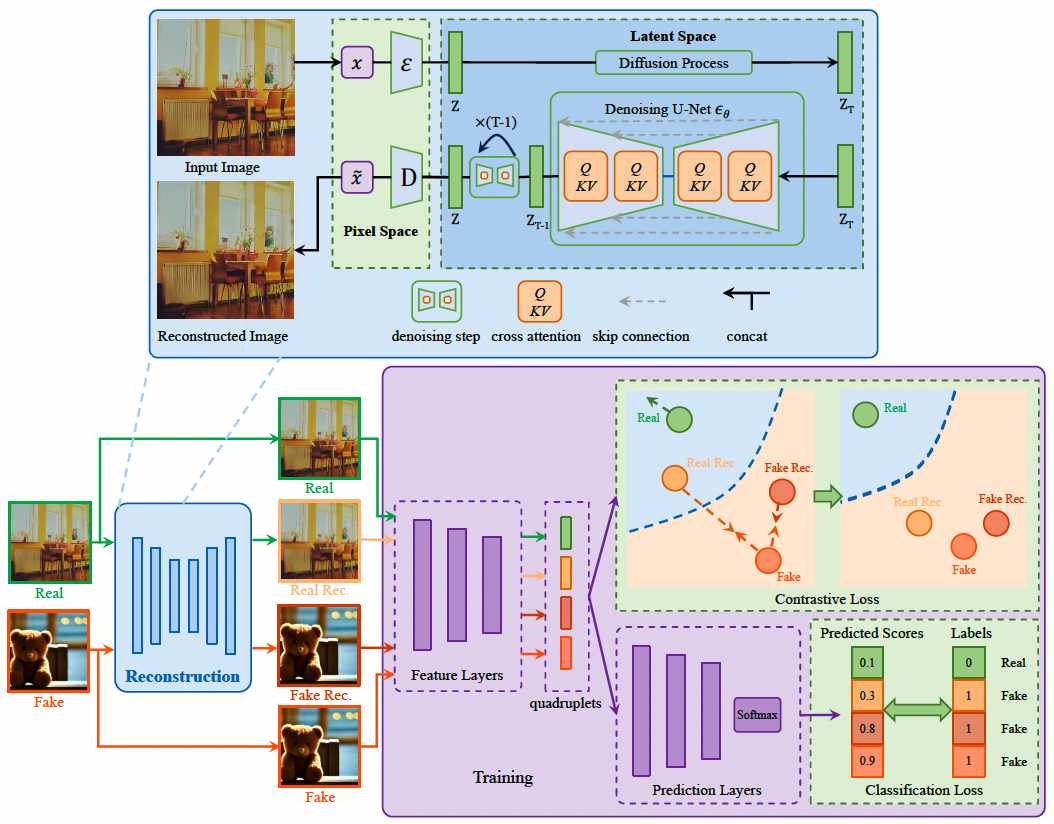
\includegraphics[width=0.4\linewidth]{DRCT.png}
      \caption{Le cadre DRCT repose sur deux étapes : d’abord, les images sont reconstruites à l’aide d’un modèle de diffusion ; ensuite, un classifieur binaire est entraîné sur les images originales et reconstruites. L’apprentissage combine une perte contrastive, pour mieux séparer les représentations réelles et générées, et une perte de classification, pour prédire si une image est réelle ou synthétique.}
      \label{fig:placeholder}
  \end{figure}  
\end{frame}

\subsection{DNF}
\begin{frame}{DNF : Diffusion Noise Feature \citep{Zhang_2025}}

\textbf{Idée principale.}
Exploiter les bruits prédits par le U-Net  à plusieurs timesteps $t_k,k=1,\dotsi,K$ comme représentations de détection.
$$
    \hat{\varepsilon}_{t_k}=\varepsilon_\theta(x_{t_k},t_k)
$$
 On a donc la sequence de bruits éstimés
$$
    \mathcal{N}(x)=\{\hat{\varepsilon}_{t_1},\hat{\varepsilon}_{t_2},\dots,\hat{\varepsilon}_{t_K}\}
$$
On fusionne ces bruits pour produire le DNF par une convolution par exemple
$$
    \operatorname{DNF}(x)=\mathcal{A}\left(\hat{\varepsilon}_{t_1},\dots,\hat{\varepsilon}_{t_K}\right)
$$
Après on utilise ce DNF pour entraîner un classifieur.
\end{frame}

\subsection{Implicit Detector}
\begin{frame}{Implicit Detector : diffusion model as detector \citep{wang}}

\textbf{Idée principale.}
Utiliser les réponses internes d’un modèle de diffusion pré-entraîné comme indices de détection.


$$
    \hat{\varepsilon}_{\text{uncond}}=\varepsilon_\theta(x_t,t,\emptyset)
$$
Et
$$
    F_t(x)=\operatorname{Concat}\left(\varepsilon,\hat{\varepsilon}_{\text{uncond}},|\varepsilon-\hat{\varepsilon}_{\text{uncond}}|\right)
$$
On fait ça pour plusieurs timestep
$$
    F(x)=\operatorname{Stack }(F_{t_1}(x),\dotsi,F_{t_K}(x))
$$
Et cet opérateur est ensuite donné à un classifieur
$$
    \hat{y}=C_\omega(F(x))
$$


\end{frame}
\begin{frame}{Implicit Detector (suite)}
    \begin{figure}
        \centering
        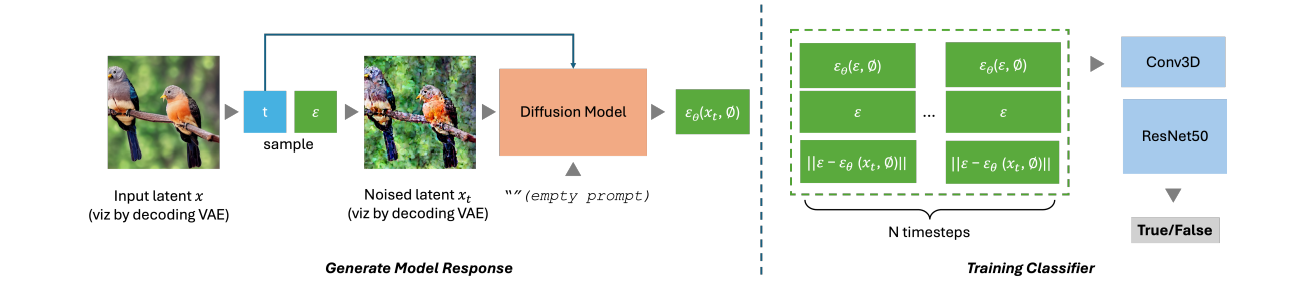
\includegraphics[width=1\linewidth]{yourmodel_detector.png}
        \caption{\textbf{Pipeline de la méthode Implicit Detector}}
        \label{fig:placeholder}
    \end{figure}
\end{frame}


\subsection{FIRE}
\begin{frame}{FIRE : Frequency-guided Reconstruction Error \citep{Chu_2025}}

\textbf{Idée principale.}
Combiner l’erreur de reconstruction avec une analyse fréquentielle.

$$
    x \longrightarrow \hat{x}=R(x)
$$
Au lieu de travailler directement avec 
$$
    E_{\text{pixel}}(x)=|x-\hat{x}|
$$
On introduit une transformation fréquentielle $\mathcal{F}(\cdot)$ et on calcule la carte d'erreur fréquentielle,
$$
    E_{\text{freq}}(x)=|\mathcal{F}(x)-\mathcal{F}(\hat{x})|
$$

Et on entraîne un classifieur sur cette carte.

\end{frame}

\subsection{LATTE}

\begin{frame}{LATTE : Latent Trajectory Embedding \citep{vasilcoiu2025lattelatenttrajectoryembedding}}

\textbf{Idée principale.}
Exploiter toute la trajectoire latente du débruitage, plutôt qu’un seul timestep ou une seule erreur.

L'image $x$ passe dans un encodeur visuel qui donne deux sorties: $ F_{\text{global}}$ une représentation globale de toute l’image et $F_{\text{vis}}$ qui est une matrice des tokens locaux qui décrivent les différentes zones de l’image.

Au lieu de regarder un seul latent bruité $z_t$, on considère la séquence,
$$
    z_T,z_{T-1},\dots,z_0
$$
 Et Chaque latent est raffiné avec des features visuelles  par cross-attention :
$$
    \tilde{z}_{t_k}=\operatorname{CrossAttn}(z_{t_k},F_{\text{vis}})
$$
La trajectoire est ensuite agrégée, par exemple par average pooling :
$$
    \Phi(x)= \operatorname{AVGPooling}(\tilde{z}_0,\dots,\tilde{z}_{T})
$$
Ensuite, cet embedding de trajectoire est concaténé avec un token global de l’image,
$$
    F_{\text{fused}}=G(F_{\text{global}},\Phi(x))
$$

\end{frame}

\begin{frame}{LATTE (suite)}
    \begin{figure}
        \centering
        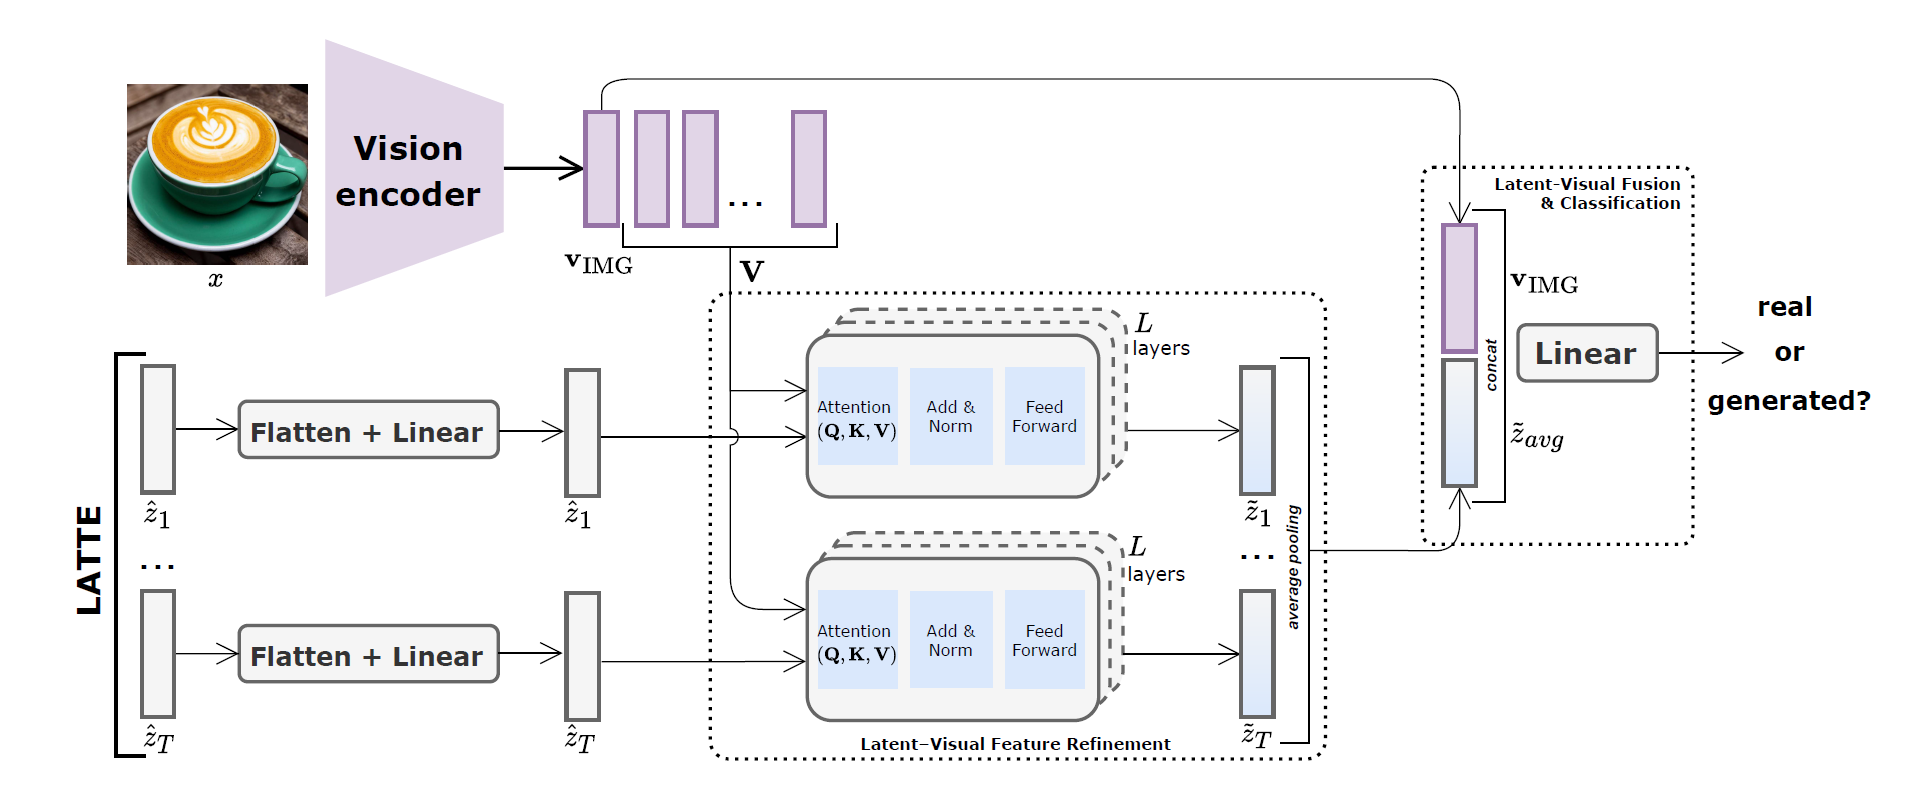
\includegraphics[width=0.8\linewidth]{latte_architecture.jpg}
        \caption{Pipeline de la Méthode LATTE}
        \label{fig:placeholder}
    \end{figure}
\end{frame}


\subsection{ANL}
\begin{frame}{ANL : Attention-guided Noise Learning \citep{qi2026deepfake}}

\textbf{Idée principale.}
Utiliser le bruit prédit par un modèle de diffusion pour guider l’attention du détecteur.

On commence par prédire le bruit ajouté à l'image $x$ au timestep $t$ par un modèle pré-entraîné
$$
    \hat{\varepsilon}_\theta=\varepsilon_\theta(x_t,t)
$$
On entraîne un détecteur à appprendre le bruit: on extrait d'abord une feature map $F$ par un backbone. Ensuite, on ajoute une entête de prédiction du bruit:
$$
\tilde{\varepsilon}=h(F)
$$
On force le détecteur à appreocher sa prédiction à celle du modèle de diffusion
$$
    \mathcal{L}_{\text{noise}}=\|\tilde{\varepsilon}-\hat{\varepsilon}_\theta\|_2^2
$$
On utilise le bruit prédit pour construire une carte d'attention:
$$
    A_{\text{noise}}=\operatorname{Attention(\tilde{\varepsilon},\hat{\varepsilon}_\theta)}
$$
Ensuite, cette attention est appliquée aux features visuelles :
$$
    F_{\text{ANL}}=A_{\text{noise}}\odot F
$$


\end{frame}
\begin{frame}{ANL (suite)}
    \begin{figure}
        \centering
        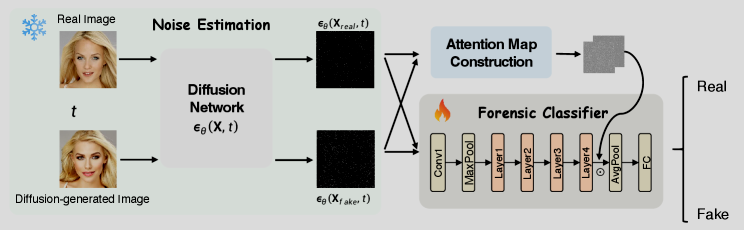
\includegraphics[width=1\linewidth]{ANL.png}
        \caption{Pipeline d'ANL}
        \label{fig:placeholder}
    \end{figure}
\end{frame}

\subsection{Tableaux}

\begin{frame}{Tableau récapitulatif}

\begin{table}
\centering
\small
\begin{tabular}{lll}
\toprule
\textbf{Famille} & \textbf{Signal exploité} & \textbf{Méthodes} \\
\midrule
Reconstruction image & \( |x-\hat{x}| \) & DIRE, AEROBLADE, FIRE \\
Erreur latente & \( |z-\hat{z}| \) & LaRE\textsuperscript{2} \\
Erreur intermédiaire & \(E_{t,\delta}\) & SeDID \\
Bruit prédit & \(\hat{\varepsilon}_\theta\) & DNF, ANL, Implicit Detector \\
Trajectoire latente & \(z_T,\dots,z_0\) & LATTE \\
\bottomrule
\end{tabular}

\caption{Synthèse des familles de méthodes exploitant les modèles de diffusion pour la détection.}
\end{table}

\end{frame}
\begin{frame}{Tableau récapitulatif (suite)}
    \newcommand{\cmark}{\checkmark}
\newcommand{\xmark}{\(\times\)}
\newcommand{\pmark}{\(\triangle\)} % partiel / indirect

\begin{table}[htbp]
\centering
\scriptsize
\renewcommand{\arraystretch}{1.15}
\begin{tabularx}{\textwidth}{
>{\raggedright\arraybackslash}p{2.8cm}
>{\centering\arraybackslash}p{1.4cm}
>{\centering\arraybackslash}p{1.7cm}
>{\centering\arraybackslash}p{1.3cm}
>{\centering\arraybackslash}p{1.4cm}
>{\centering\arraybackslash}p{1.4cm}
}
\toprule
\textbf{Méthode} 
& \textbf{Reconstr.} 
& \textbf{Bruit / U-Net} 
& \textbf{Latent} 
& \textbf{Multi-\(t\)}
& \textbf{Hybride} \\
\midrule

\textbf{DIRE} 
& \cmark 
& \pmark 
& \xmark 
& \pmark 
& \xmark \\

\textbf{SeDID} 
& \pmark 
& \cmark 
& \xmark 
& \cmark 
& \pmark \\

\textbf{DNF} 
& \xmark 
& \cmark 
& \pmark 
& \cmark 
& \pmark \\

\textbf{AEROBLADE} 
& \cmark 
& \xmark 
& \cmark 
& \xmark 
& \xmark \\

\textbf{LaRE\textsuperscript{2}} 
& \cmark 
& \cmark 
& \cmark 
& \pmark 
& \cmark \\

\textbf{DRCT} 
& \cmark 
& \pmark 
& \pmark 
& \pmark 
& \cmark \\

\textbf{Implicit Detector} 
& \xmark 
& \cmark 
& \cmark 
& \cmark 
& \pmark \\


\textbf{FIRE} 
& \cmark 
& \pmark 
& \pmark 
& \pmark 
& \cmark \\

\textbf{LATTE} 
& \pmark 
& \cmark 
& \cmark 
& \cmark 
& \cmark \\

\textbf{ANL} 
& \xmark 
& \cmark 
& \pmark 
& \pmark 
& \cmark \\

\bottomrule
\end{tabularx}
\caption{Comparaison synthétique des méthodes exploitant les modèles de diffusion pour la détection de deepfakes. Le symbole \(\checkmark\) indique que la caractéristique est centrale dans la méthode, \(\times\) indique qu’elle n’est pas utilisée, et \(\triangle\) indique une utilisation partielle ou indirecte. La colonne \textit{Hybride} indique si la méthode combine un signal issu de la reconstruction ou du bruit de diffusion avec une autre technique, comme l’attention, l’analyse fréquentielle, l’apprentissage contrastif ou un classifieur dédié.}
\label{tab:comparison_diffusion_detection_methods}
\end{table}
\end{frame}


%%%%%%%%%%%%%%%%%%%%%%%%%%%%%%%%%%%%%%%%%%%%%%%%%%%%%%%%%%%%%%%%%%%%

\section{Bases de données}
\begin{frame}{Bases de données}
    $\to$ Les premières bases de données dédiés à la détection de deepfakes étaient surtout générés par des GANs (réseaux antagonistes génératifs) ou des autoencodeurs.

    \bigskip

    $\to$ L'évolution des modèles de diffusion produisant des deepfakes plus réalistes rend nécessaire l'introduction de bases de données générées exclusivement par diffusion.

    \bigskip 
    
    $\to$ 3 catégories : 
    \begin{itemize}
        \item benchmarks de deepfakes faciaux,
        \item benchmarks plus généralistes de vidéos générées par intelligence artificielle,
        \item bases de données issues de contenus réels collectés.
    \end{itemize}
\end{frame}

\begin{frame}{DigiFakeAV \citep{liu}}
    $\to$ Benchmark récent de vidéos deepfakes générées par modèles de diffusion, comme par exemple Sonic \citep{ji}.

    \bigskip

    $\to$ 60 000 vidéos : 
    \begin{itemize}
        \item 50 000 vidéos fakes,
        \item 10 000 vidéos réelles.
    \end{itemize}

    \bigskip 

    $\to$ Avantages : 
    \begin{itemize}
        \item Génération exclusivement faite par modèles de diffusion,
        \item Diversité ethnique et de genre,
        \item qualité visuelle élevée.
    \end{itemize}
\end{frame}

\begin{frame}{TalkingHeadBench \citep{xiong}}
    $\to$ Autre benchmark récent de vidéos deepfakes de types "têtes parlantes" dont certaines générées par modèles de diffusion (Hallo \citep{xu2024} ou encore AniPortrait \citep{wei}).

    \bigskip

    $\to$ 2 994 vidéos fake issues de huit générateurs différents, 2 312 vidéos réelles.

    \bigskip

    $\to$ Il a fait objet d'un processus de sélection afin d'éliminer les deepfakes présentant des artéfacts trop évidents.

    \bigskip

    $\to$ Particulièrement intéressant pour tester la capacité de généralisation des détecteurs, c'est-à-dire leur aptitude à rester efficace face à l'inconnu.
\end{frame}

\begin{frame}{MAVOS-DD \citep{croitoru}}
    $\to$ Benchmark multimodal conçu pour la détection de deepfake audio-visuels.

    \bigskip

    $\to$ Plus de 250 heures de vidéos réelles et fake (91h de vidéos réelles et 161h de fakes) générées à partir de plusieurs familles de modèles génératifs, incluant certains modèles de diffusion.

    \bigskip

    $\to$ Principal intêret : son approche open-set, c'est-à-dire que les modèles de détection sont évalués sur des types de deepfakes qui n’ont pas forcément été observés pendant la phase d'entraînement.

    \bigskip

    $\to$ Inconvénient : Les modèles génératifs ne sont pas exclusivement des modèles de diffusion. 
\end{frame}

\begin{frame}{GenVidBench \citep{ni}}
    $\to$ Benchmark de vidéos générées par l'intelligence artificielle, principalement à partir de scénarios text-to-video et image-to-video.

    \bigskip

    $\to$ Avec plus de 143 000 vidéos, c'est l'un des plus vastes benchmarks de contenu IA général (personnes, animaux, plantes...). Cependant, seulement 9,5\% de vidéos avec des humains, et pas spécifiquement des deepfakes.

    \bigskip

    $\to$ Inclut des vidéos générées par différents modèles de diffusion récents tels que Stable Video Diffusion \citep{blattmann}, ou VideoCrafter2 \citep{chen2}.

    \bigskip

    $\to$ Approche "cross-source" et "cross-generator" : les sources de génération (prompts ou images) et les générateurs diffèrent entre l'entraînement et le test.
\end{frame}

\begin{frame}{Political Deepfakes Incidents Database (PDID) \citep{walker}}
    $\to$ Véritables incidents politiques de deepfakes et "cheapfakes". \\
    "cheapfakes" : contenus réels modifiés par des techniques simples comme des montages, qui ne sont pas générés par l'intelligence artificielle.

    \bigskip 

    $\to$ contenus du monde réel collectés depuis 2017 (personnalités politiques majeures, évènements géopolitiques mondiaux).

    \bigskip

    $\to$ Les chercheurs ont précisé dans quel but les deepfakes ont été générés (blague, truquage, etc.) et quels ont été leurs effets réels.

    \bigskip 

    $\to$ Les modèles utilisés pour la génération ne sont pas précisés, mais son utilisation peut être intéressante pour tester les modèles de détection avec des deepfakes qui ont vraiment été utilisés à des fins malveillantes.
\end{frame}

\begin{frame}{Datasets d'images complémentaires}
    Encore peu de bases de données vidéos exclusivement générés par diffusion, il est donc utile de citer des datasets d'images, qui peuvent permettre d’étudier les signatures intrinsèques des modèles de diffusion, qui peuvent être retrouvées dans les vidéos.

    \bigskip

    \begin{itemize}
        \item GenImage \citep{zhu2023genimage} : benchmark massif d'images générées par des GANs et des modèles de diffusion, contenant des deepfakes, des images d'animaux ou encore des paysages.
        \item DeepFakeFace \citep{song} : dataset de deepfakes de célébrités générés par diffusion, créé pour entraîner et tester des algorithmes de détection de deepfake.
        \item DiFF \citep{cheng} : base de données de plus de 500 000 visages fake générés par 13 modèles de diffusion. Les auteurs proposent également une méthode de détection basée sur les graphes de contours.
        \item DiffusionFace \citep{chen} : jeu de données de deepfakes générés par diffusion, regroupant 600 000 images de haute qualité générées par 11 modèles différents.
    \end{itemize}
\end{frame}

%%%%%%%%%%%%%%%%%%%%%%%%%%%%%%%%%%%%%%%%%%%%%%%%%%%%%%%%%%%%%%%%%%%%

\section{Expérimentations}
\subsection{Comparaison de deux méthodes}
\begin{frame}{Expérimentation 1 : U-Net multi-\(t\) sur CIFAKE}


\textbf{Principe.}
Pour une image \(x\), on l’encode d’abord dans l’espace latent :

$$
    z_0=\mathcal{E}(x)
$$

Puis, pour plusieurs timesteps $t_1,\dots,t_K$, on ajoute du bruit :
$$
    z_{t_k}=\sqrt{\alpha_{t_k}}z_0+\sqrt{1-\alpha_{t_k}}\varepsilon
$$

Le U-Net prédit ensuite le bruit ajouté et On construit alors une carte d’erreur :

$$
    M_{t_k}=|\varepsilon-\hat{\varepsilon}_{t_k}|
$$

\vspace{0.2cm}

\begin{block}{Signal utilisé}
Les cartes d’erreur obtenues à plusieurs timesteps sont empilées pour former l’entrée du classifieur :
$$
    M(x)=\operatorname{Stack}(M_{t_1},\dots,M_{t_K})
$$
\end{block}

\end{frame}

\begin{frame}{Expérimentation 2 : LCM \citep{luo2023latentconsistencymodelssynthesizing} sur CIFAKE}


\textbf{Principe.}
Comme précédemment, l’image est d’abord encodée dans l’espace latent On ajoute ensuite du bruit au latent :
$$
    z_t=\sqrt{\alpha_t}z_0+\sqrt{1-\alpha_t}\varepsilon
$$

Le LCM effectue quelques étapes rapides de débruitage et produit une estimation du latent propre :

$$
    \hat{z}_0
$$

On calcule alors une erreur de reconstruction latente :

$$
    M_{\text{LCM}}(x)=|z_0-\hat{z}_0|
$$

\vspace{0.2cm}

\begin{block}{Signal utilisé}
Contrairement à l’approche U-Net multi-\(t\), qui compare le bruit réel et le bruit prédit, l’approche LCM compare le latent original et le latent reconstruit.
\end{block}
\end{frame}

\begin{frame}{Expérimentation  : comparaison des résultats}

\begin{table}
\centering
\small
\begin{tabular}{lccccc}
\toprule
\textbf{Méthode} & \textbf{Acc.} & \textbf{Préc.} & \textbf{Recall} & \textbf{F1} & \textbf{AUC} \\
\midrule
U-Net multi-\(t\) + CNN & 0.67 & 0.61 & 0.96 & 0.74 & 0.86 \\
LCM + CNN               & 0.80 & 0.81 & 0.78 & 0.80 & 0.87 \\
\bottomrule
\end{tabular}
\caption{Comparaison des deux approches sur un sous-ensemble de CIFAKE(2000 images d'entraînement, 500 de validation et 100 de test).}
\end{table}

%U-Net multi-\(t\) détecte presque tous les fake, mais produit beaucoup de faux positifs.  
%LCM + CNN offre un meilleur compromis global entre précision, rappel et F1-score.
 \begin{figure}
     \centering
     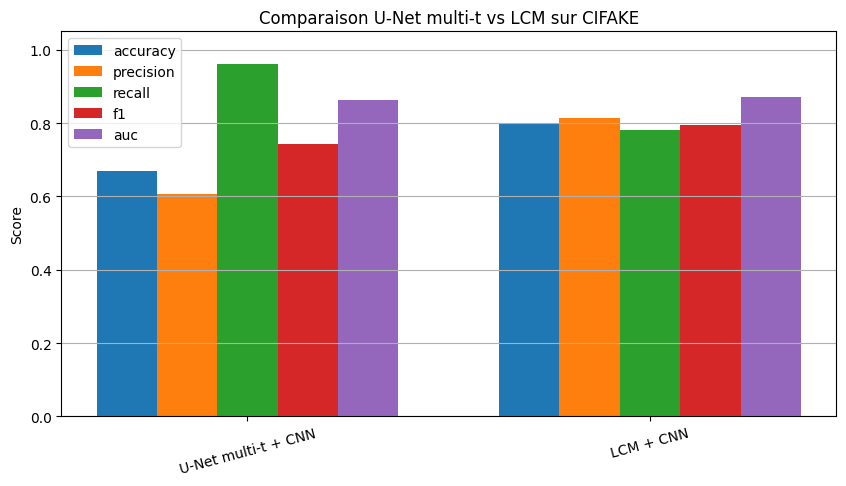
\includegraphics[width=0.5
     \linewidth]{u_net_vs_lcm_cifake.png}
     \caption{C}
     \label{fig:placeholder}
 \end{figure}

\end{frame}

\subsection{Extraction du graphe du visage}

\begin{frame}{Extraction du graphe du visage}
    $\to$ Méthode utilisée : Bibliothèque MediaPipe, Module Face Mesh \\
    Permet d'obtenir un maillage facial détaillé avec 468 sommets.

    \bigskip

    $\to$ Génération d'une vidéo avec suivi du graphe du visage en temps réel.

    \begin{figure}
        \centering
        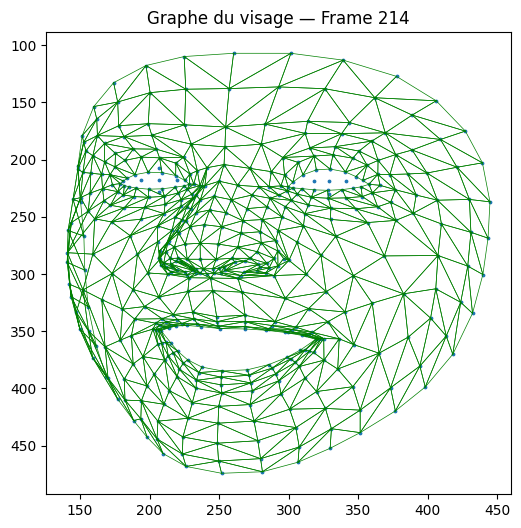
\includegraphics[width=0.32\linewidth]{exemple de graphe du visage.png}
        \caption{Graphe du visage extrait d'une vidéo fake du dataset TalkingHeadBench}
        \label{fig:facegraph}
    \end{figure}
    
\end{frame}

\section{Connaissances acquises}

\begin{frame}{Modèles de diffusion}
    $\to$ Modèles génératifs qui permettent de produire ou de traiter une image en effectuant un processus de débruitage.

    \bigskip

    $\to$ Deux étapes :
    \begin{itemize}
        \item Processus direct : le modèle commence par prendre une donnée réelle puis y ajoute progressivement du bruit, souvent Gaussien, jusqu'à obtenir une image de bruit pur.
        \item Processus inverse : un réseau de neurones est entraîné à faire le chemin inverse, il doit apprendre à prédire et à retirer le bruit pour générer des contenus réalistes.
    \end{itemize}

    \bigskip 

    $\to$ Exemples : Stable Diffusion \citep{rombach2022highresolutionimagesynthesislatent}, Midjourney \citep{midjourney2022}, DALLE-2 \citep{ramesh}.
    
    \bigskip

    $\to$ Pour accélerer le processus, les LDM (Latent Diffusion Models \citep{rombach2022highresolutionimagesynthesislatent}) ont été développés. Au lieu de travailler directement sur les pixels de l'image, ils travaillent dans un espace latent, ce qui permet de générer des images beaucoup plus efficacement.
\end{frame}

\begin{frame}{La détection}
    $\to$ Les modèles de diffusions sont déjà des détecteurs implicites car leurs réponses internes face à une image bruitée révèlent des différences entre images réelles et synthétiques \citep{wang}

    \bigskip
    
    $\to$ Les approches récentes les plus performantes, on retrouve DRCT,FIRE,LATTE et ANL. Ces méthodes dépassent les approches fondées uniquement sur une erreur de reconstruction simple, en combinant la reconstruction ou le bruit de diffusion   avec d'autres mécanismes: apprentissage contrastif, analyse fréquentielle, trajectoire latente, attention guidée ou guidage par Stable Diffusion.
\end{frame}

\section{Références}
\begin{frame}[allowframebreaks]{Références}
\bibliographystyle{plainnat}
\bibliography{Ref}
\end{frame}
\end{document}